\openchapterblock

%\chapter{Data Provenance for Sport}
\chapter{Computational Pipelines}

\section{Symbols for Custom Sport Provenance Notation}
\label{appendixsec:SportSymbols}

\begin{table}[htpb]
\caption{Specialised symbols for Entities}
\label{SportSymbolsEntity}
\begin{tabular}{p{4cm}p{7cm}r}
\toprule
\textbf{Semantic\newline Construct\newline (W3C PROV)} & \textbf{Specialised Symbol\newline(for Sport)} & \textbf{ID} \\
\midrule
\multirow{4}{*}{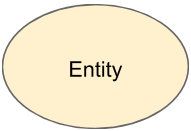
\includegraphics[width=3cm]{figs/prov_symbols/prov-entity.png}}      & \begin{tabular}[t]{@{}l@{}}Video feed\\ 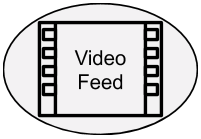
\includegraphics[width=3cm]{figs/prov_symbols/a_vidfeed.png}\end{tabular}                   & 1  \\
\cline{2-3}
                             & \begin{tabular}[t]{@{}l@{}}Game state\\ 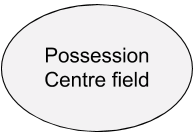
\includegraphics[width=3cm]{figs/prov_symbols/b_state.png}\end{tabular}                                                                         & 2  \\
\cline{2-3}
                             & \begin{tabular}[t]{@{}l@{}}Game event\\ 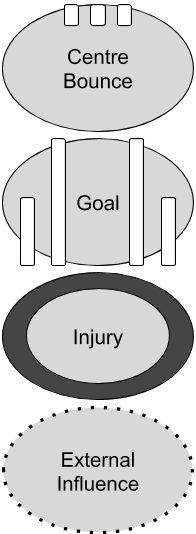
\includegraphics[width=3cm]{figs/prov_symbols/c_event.png}\end{tabular}                                                                        & 3  \\
\cline{2-3}
                             & \begin{tabular}[t]{@{}l@{}}Metric             \\ 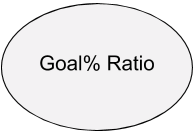
\includegraphics[width=3cm]{figs/prov_symbols/d_metric.png}\end{tabular}                                                                       & 4  \\
\bottomrule
\end{tabular}
\end{table}

\begin{table}[htpb]
\caption{Specialised symbols for Activities}
\label{SportSymbolsActivity}
\begin{tabular}{p{4cm}p{7cm}r}
\toprule
\textbf{Semantic\newline Construct\newline (W3C PROV)} & \textbf{Specialised Symbol\newline(for Sport)} & \textbf{ID} \\
\midrule
\multirow{4}{*}{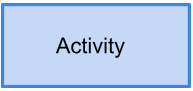
\includegraphics[width=3cm]{figs/prov_symbols/prov-activity.png}}      & \begin{tabular}[t]{@{}l@{}}Physical action\\ 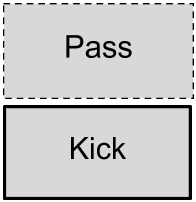
\includegraphics[width=3cm]{figs/prov_symbols/e_action.png}\end{tabular}                   & 5  \\
\cline{2-3}
                             & \begin{tabular}[t]{@{}l@{}}Manual process\\ 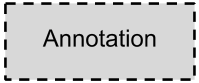
\includegraphics[width=3cm]{figs/prov_symbols/f_manual.png}\end{tabular}                                                                         & 6  \\
\cline{2-3}
                             & \begin{tabular}[t]{@{}l@{}}Computation\\ 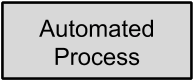
\includegraphics[width=3cm]{figs/prov_symbols/g_comp.png}\end{tabular}                                                                        & 7  \\
\cline{2-3}
                             & \begin{tabular}[t]{@{}l@{}}De-identification             \\ 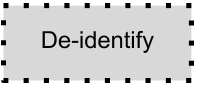
\includegraphics[width=3cm]{figs/prov_symbols/h_deident.png}\end{tabular}                                                                       & 8  \\
\bottomrule
\end{tabular}
\end{table}

\begin{table}[htpb]
\caption{Specialised symbols for Agents}
\label{SportSymbolsAgent}
\begin{tabular}{p{4cm}p{7cm}r}
\toprule
\textbf{Semantic\newline Construct\newline (W3C PROV)} & \textbf{Specialised Symbol\newline(for Sport)} & \textbf{ID} \\
\midrule
\multirow{4}{*}{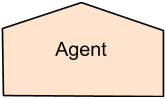
\includegraphics[width=3cm]{figs/prov_symbols/prov-agent.png}}      & \begin{tabular}[t]{@{}l@{}}Analyst / System\\ 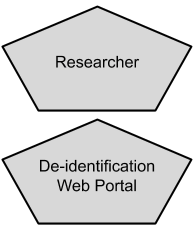
\includegraphics[width=3cm]{figs/prov_symbols/i_analyst.png}\end{tabular}                   & 9  \\
\cline{2-3}
                             & \begin{tabular}[t]{@{}l@{}}Player / Role\\ 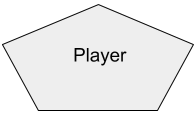
\includegraphics[width=3cm]{figs/prov_symbols/j_player.png}\end{tabular}                                                                         & 10  \\
\cline{2-3}
                             & \begin{tabular}[t]{@{}l@{}}Team\\ 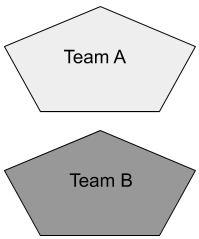
\includegraphics[width=3cm]{figs/prov_symbols/k_team.png}\\ (Distinguished by colour)\end{tabular}                                                                        & 11  \\
\cline{2-3}
                             & \begin{tabular}[t]{@{}l@{}}Sensor             \\ 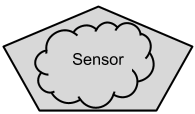
\includegraphics[width=3cm]{figs/prov_symbols/l_sensor.png}\end{tabular}                                                                       & 12  \\
\bottomrule
\end{tabular}
\end{table}

\begin{table}[htpb]
\caption{Specialised symbols for Associations}
\label{SportSymbolsAssoc}
\begin{tabular}{p{4cm}p{7cm}r}
\toprule
\textbf{Semantic\newline Construct\newline (W3C PROV)} & \textbf{Specialised Symbol\newline(for Sport)} & \textbf{ID} \\
\midrule
\multirow{2}{*}{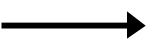
\includegraphics[width=3cm]{figs/prov_symbols/m_assoc.png}}      & \begin{tabular}[t]{@{}l@{}}Data dependency\\ 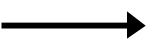
\includegraphics[width=3cm]{figs/prov_symbols/m_assoc.png}\\ (Distinguished by context)\end{tabular}                   & 13  \\
\cline{2-3}
                                                                                 & \begin{tabular}[t]{@{}l@{}}Physical causality\\ 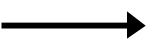
\includegraphics[width=3cm]{figs/prov_symbols/m_assoc.png}\\ (Distinguished by context)\end{tabular}                   & 14  \\
\bottomrule
\end{tabular}
\end{table}

\begin{table}[htpb]
\caption{Specialised symbols for Bundles}
\label{SportSymbolsBundle}
\begin{tabular}{p{4cm}p{7cm}r}
\toprule
\textbf{Semantic\newline Construct\newline (W3C PROV)} & \textbf{Specialised Symbol\newline(for Sport)} & \textbf{ID} \\
\midrule
\multirow{1}{*}{Bundle (no symbol)}      & \begin{tabular}[t]{@{}l@{}}Group\\ 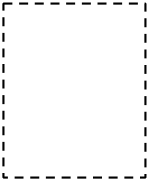
\includegraphics[width=3cm]{figs/prov_symbols/n_group.png}\end{tabular}                   & 15  \\
\bottomrule
\end{tabular}
\end{table}

\clearpage

\section{Effectiveness of visual notation against principles of Physics of Notations}

{
\renewcommand{\arraystretch}{1.8} % vertical cell spacing
\begin{longtable}[c]{@{}lll@{}}
\caption{Effectiveness of visual notation against principles of Physics of Notations \cite{Moody2009}}
\label{appendix:tab:EvalNotation}\tabularnewline
\hline
\endhead
\toprule
\begin{minipage}[t]{0.30\columnwidth}\raggedright\strut
{\textbf{Criterion}}
\strut\end{minipage} &
\begin{minipage}[t]{0.30\columnwidth}\raggedright\strut
{\textbf{W3C PROV}}
\strut\end{minipage} &
\begin{minipage}[t]{0.30\columnwidth}\raggedright\strut
{\textbf{VisTrails}}
\strut\end{minipage}\tabularnewline
\midrule
\begin{minipage}[t]{0.30\columnwidth}\raggedright\strut
{Semiotic Clarity}{\\
}{(fraction of semantic constructs in Table \ref{Params} mapped to
unique symbols)}
\strut\end{minipage} &
\begin{minipage}[t]{0.30\columnwidth}\raggedright\strut
{4/15}

{}

{Contains high level semantics for entity, activity, agent and
association.}
\strut\end{minipage} &
\begin{minipage}[t]{0.30\columnwidth}\raggedright\strut
{3/15}

{}

{Metric (port), computation, data dependency (association).}

{}

No concept of agents. No ability to directly model real world. No
concept of physical causality.
\strut\end{minipage}\tabularnewline
\begin{minipage}[t]{0.30\columnwidth}\raggedright\strut
{Perceptual Discriminabilit}{y}{~\\
}{(fraction of symbols }{with unique visual variables}{)}
\strut\end{minipage} &
\begin{minipage}[t]{0.30\columnwidth}\raggedright\strut
{4/4}

{}

{Could be improved: different }{colours / shapes}{~for specialisations.
(Points still awarded because top level constructs have distinct
symbols)}
\strut\end{minipage} &
\begin{minipage}[t]{0.30\columnwidth}\raggedright\strut
{3/3}

{}

{Ports and activities share same shape as each other, but differ by
size.}

{}

{Could be improved: ports with different types should have different
colours / shapes. Activities with different types should have different
colours and use a larger variety of shapes. (Points still awarded for
these because only one type of sport semantic construct was supported)}
\strut\end{minipage}\tabularnewline
\begin{minipage}[t]{0.30\columnwidth}\raggedright\strut
{Semantic Transparency\\
}{(fraction of symbols with obvious meanings)}
\strut\end{minipage} &
\begin{minipage}[t]{0.30\columnwidth}\raggedright\strut
{0/4}

{}

{Use of circles for entities and rectangles for processes conflicts with
data flow diagrams (which use circles for processes). Use of house
shaped pentagons for agents is only memorable when agent represents an
organisation. Arrows are in direction of data dependency, but intuitive
interpretation is in direction of data flow.}
\strut\end{minipage} &
\begin{minipage}[t]{0.30\columnwidth}\raggedright\strut
{3/3}

{}

{Analogy: electric circuit (rectangular components, small contacts,
connection wires)}

{}

{Could be improved: while obvious square is a port, not obvious which
port is which (user has to memorise order). While obvious that box is a
process, specific type of process is not obvious (e.g. uses pentagon for
control flow rather than conventional diamond for ``if'' condition)}
\strut\end{minipage}\tabularnewline
\begin{minipage}[t]{0.30\columnwidth}\raggedright\strut
{Complexity Management\\
}{(can it visualize complex workflows?)}
\strut\end{minipage} &
\begin{minipage}[t]{0.30\columnwidth}\raggedright\strut
{Yes}

{}

{Ontologies support the ``Open-world assumption'', thus allowing
specifying as much or as little detail as appropriate.}
\strut\end{minipage} &
\begin{minipage}[t]{0.30\columnwidth}\raggedright\strut
{Yes}

{}

{Supports grouping nodes}
\strut\end{minipage}\tabularnewline
\begin{minipage}[t]{0.30\columnwidth}\raggedright\strut
{Cognitive Integration}{\\
}{(can the user navigate without getting lost?)}
\strut\end{minipage} &
\begin{minipage}[t]{0.30\columnwidth}\raggedright\strut
{Yes}

{}

{Includes concept of ``bundles'' to annotate information required to
navigate documents at meta-level. E.g. to describe provenance of
provenance information.}
\strut\end{minipage} &
\begin{minipage}[t]{0.30\columnwidth}\raggedright\strut
{Yes}

{}

{Top level workflow acts as overview, then user can drill down into
parameter values, history variations, etc.}
\strut\end{minipage}\tabularnewline
\begin{minipage}[t]{0.30\columnwidth}\raggedright\strut
{Visual Expressiveness}{\\
(fraction of visual variables used)}
\strut\end{minipage} &
\begin{minipage}[t]{0.30\columnwidth}\raggedright\strut
{2/8}

{}

{Shape and colour.}
\strut\end{minipage} &
\begin{minipage}[t]{0.30\columnwidth}\raggedright\strut
{1/8}

{}

{Shape}

{}

{Colour is used for execution state, but this is not one of semantic
constructs, and brightness is used to determine if a port is connected,
but neither of these map to semantic constructs of relevance.}
\strut\end{minipage}\tabularnewline
\begin{minipage}[t]{0.30\columnwidth}\raggedright\strut
{Dual Coding}{\\
(fraction of symbol parameters with multiple unique visual variables)}
\strut\end{minipage} &
\begin{minipage}[t]{0.30\columnwidth}\raggedright\strut
{1/3}

{}

{Shape and colour used together to ensure symbols are distinct (i.e.
colours improve distinguishability of symbols, and even if user is
colour blind, symbols are still distinguishable by shape)}
\strut\end{minipage} &
\begin{minipage}[t]{0.30\columnwidth}\raggedright\strut
{0/3}

{}

{In theory shape and colour can be assigned if designing custom module,
but colour is not used in any of the default modules.}
\strut\end{minipage}\tabularnewline
\begin{minipage}[t]{0.30\columnwidth}\raggedright\strut
{Graphic Economy}{\\
(total symbols, less is better as it reduces cognitive load)}
\strut\end{minipage} &
\begin{minipage}[t]{0.30\columnwidth}\raggedright\strut
{4}
\strut\end{minipage} &
\begin{minipage}[t]{0.30\columnwidth}\raggedright\strut
{3}

{}

{(If all features not part of assessment were removed)}
\strut\end{minipage}\tabularnewline
\begin{minipage}[t]{0.30\columnwidth}\raggedright\strut
{Cognitive Fit}{\\
(is the notation understandable to performance analysts?)}
\strut\end{minipage} &
\begin{minipage}[t]{0.30\columnwidth}\raggedright\strut
{Partial}

{}

{When arrows are labelled, visual notation is unambiguous.}
\strut\end{minipage} &
\begin{minipage}[t]{0.30\columnwidth}\raggedright\strut
{Partial}

{}

{Intuitive flow metaphor; however, advanced operations require writing
custom Python scripts.}
\strut\end{minipage}\tabularnewline
\bottomrule
\end{longtable}
}






\clearpage

\section{Usability evaluation of VisTrails using Nielsen's top ten heuristics}

{
\renewcommand{\arraystretch}{1.8} % vertical cell spacing
\begin{longtable}[c]{@{}lll@{}}
% https://www.nngroup.com/articles/ten-usability-heuristics/
\caption{Usability evaluation of VisTrails using
Nielsen's top ten heuristics \cite{Nielsen1994}}
\label{appendix:tab:EvalUsability}\tabularnewline
\hline
\endhead
\toprule
\begin{minipage}[t]{0.30\columnwidth}\raggedright\strut
{\textbf{Criterion}}
\strut\end{minipage} &
\begin{minipage}[t]{0.30\columnwidth}\raggedright\strut
{\textbf{Support}}
\strut\end{minipage} &
\begin{minipage}[t]{0.30\columnwidth}\raggedright\strut
{\textbf{Issues}}
\strut\end{minipage}\tabularnewline
\midrule
\begin{minipage}[t]{0.30\columnwidth}\raggedright\strut
{Visibility of system status}
\strut\end{minipage} &
\begin{minipage}[t]{0.30\columnwidth}\raggedright\strut
{Shows progress indicator when evaluating workflow. Displays which
modules executed / have errors.}
\strut\end{minipage} &
\begin{minipage}[t]{0.30\columnwidth}\raggedright\strut
{}
\strut\end{minipage}\tabularnewline
\begin{minipage}[t]{0.30\columnwidth}\raggedright\strut
{Match between system and the real world}
\strut\end{minipage} &
\begin{minipage}[t]{0.30\columnwidth}\raggedright\strut
{Boxes for processes connected by lines resembles real-world electronic
wiring of modules.}
\strut\end{minipage} &
\begin{minipage}[t]{0.30\columnwidth}\raggedright\strut
{Some terms may present confusion for non-technical users:
``PythonCalc'' (evaluate an expression), ``StandardOutput'' (display
result in the terminal), and ``Map'' (a higher order function, not a
geographical map).}
\strut\end{minipage}\tabularnewline
\begin{minipage}[t]{0.30\columnwidth}\raggedright\strut
{User control and freedom}
\strut\end{minipage} &
\begin{minipage}[t]{0.30\columnwidth}\raggedright\strut
{Full tracking of history as tree}
\strut\end{minipage} &
\begin{minipage}[t]{0.30\columnwidth}\raggedright\strut
{}
\strut\end{minipage}\tabularnewline
\begin{minipage}[t]{0.30\columnwidth}\raggedright\strut
{Consistency and standards}
\strut\end{minipage} &
\begin{minipage}[t]{0.30\columnwidth}\raggedright\strut
{}
\strut\end{minipage} &
\begin{minipage}[t]{0.30\columnwidth}\raggedright\strut
{Some terms such as ``port'' (rather than input / output) may increase
time to learn.}
\strut\end{minipage}\tabularnewline
\begin{minipage}[t]{0.30\columnwidth}\raggedright\strut
{Error prevention}
\strut\end{minipage} &
\begin{minipage}[t]{0.30\columnwidth}\raggedright\strut
{Ports have types to ensure that user can only connect two ports if
their types match.}
\strut\end{minipage} &
\begin{minipage}[t]{0.30\columnwidth}\raggedright\strut
{}
\strut\end{minipage}\tabularnewline
\begin{minipage}[t]{0.30\columnwidth}\raggedright\strut
{Recognition rather than recall}
\strut\end{minipage} &
\begin{minipage}[t]{0.30\columnwidth}\raggedright\strut
{The system provides some support to aid the user's memory (e.g. dark
ports to remind the user a default has been set)}
\strut\end{minipage} &
\begin{minipage}[t]{0.30\columnwidth}\raggedright\strut
{The user needs to memorise}{~}{the port order of modules to use the
interface efficiently.}
\strut\end{minipage}\tabularnewline
\begin{minipage}[t]{0.30\columnwidth}\raggedright\strut
{Flexibility and efficiency of use}
\strut\end{minipage} &
\begin{minipage}[t]{0.30\columnwidth}\raggedright\strut
{Provides shortcut key combinations for advanced users}
\strut\end{minipage} &
\begin{minipage}[t]{0.30\columnwidth}\raggedright\strut
{}
\strut\end{minipage}\tabularnewline
\begin{minipage}[t]{0.30\columnwidth}\raggedright\strut
{Aesthetic and minimalist design}
\strut\end{minipage} &
\begin{minipage}[t]{0.30\columnwidth}\raggedright\strut
{Main focus of the application is on the workflow}
\strut\end{minipage} &
\begin{minipage}[t]{0.30\columnwidth}\raggedright\strut
{}
\strut\end{minipage}\tabularnewline
\begin{minipage}[t]{0.30\columnwidth}\raggedright\strut
{Help users recognise, diagnose, and recover from errors}
\strut\end{minipage} &
\begin{minipage}[t]{0.30\columnwidth}\raggedright\strut
{System highlights module(s) with error}
\strut\end{minipage} &
\begin{minipage}[t]{0.30\columnwidth}\raggedright\strut
{Use of colour as sole indicator of error could be problematic for users
with colour blindness.}
\strut\end{minipage}\tabularnewline
\begin{minipage}[t]{0.30\columnwidth}\raggedright\strut
{Help and documentation}
\strut\end{minipage} &
\begin{minipage}[t]{0.30\columnwidth}\raggedright\strut
{User manual includes step-by-step guidelines on how to use.}


{}

{In-built option to display documentation for the selected module}
\strut\end{minipage} &
\begin{minipage}[t]{0.30\columnwidth}\raggedright\strut
{In-built documentation for module often missing}
\strut\end{minipage}\tabularnewline
\bottomrule
\end{longtable}
}

\closechapterblock
